\documentclass[iop]{emulateapj}
\usepackage{graphicx,pdfpages}
\usepackage{color}

\newcommand{\hilight}[1]{\colorbox{yellow}{#1}}
\newcommand{\teff}{\mbox{$T_{\rm eff}$}}
\newcommand{\chisq}{\mbox{$\chi^{2}$}}
\newcommand{\fmod}{\mbox{$f_{mod,i}$}}
\newcommand{\fobs}{\mbox{$f_{obs,i}$}}
\newcommand{\vij}{\mbox{$V_{ij}$}}
\newcommand{\bj}{\mbox{$B_{j}$}}
\newcommand{\sigi}{\mbox{$\sigma_{i}$}}


\begin{document}
\title{Eclipse Mapping Code}
\author{Woody Austin}

\begin{abstract}
I describe a C code that can read in time series photometry data of a transiting planet host star and produce a two dimensional surface brightness map of it. Using the Nelder-Mead Simplex Algorithm to minimize a chi-squared function, I am able to solve for relative brightness on the surface of the star. This code is meant to be easily extensible to any Kepler object. Planetary transits in the Kepler data allow for higher resolution of this brightness map along the path of the transit.
\end{abstract}
\maketitle

\section{Introduction \label{intro}}
\vspace{9mm}

\section{Description of the Model \label{description}}
Overall characterization of the necessary pieces of information. This includes terminology, geometry of a star in the general case, input parameters, model flux, limb darkening, and a description of the brightness values for which we are solving.
%\begin{figure}[h]
%	\centering
%	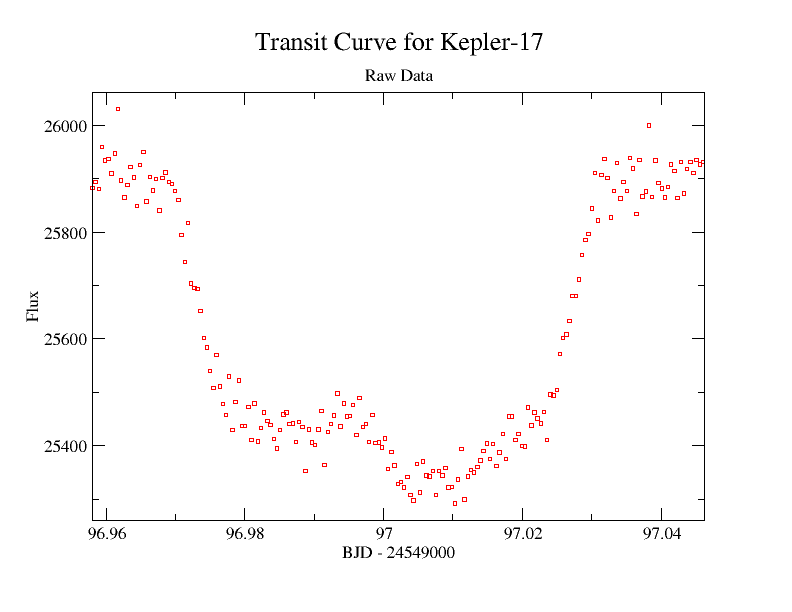
\includegraphics[width=.5\textwidth]{images/k17trans.png}
%	\caption{One transit from the actual Kepler 17 light curve. You can see the characteristic "bite" out of the transit curve where a starspot is likely occluded.}
%	\label{k17trans}
%\end{figure}
%\begin{figure}[h]
%	\centering
%	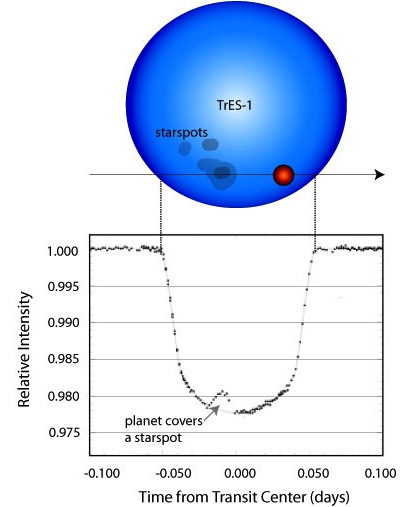
\includegraphics[width=.5\textwidth]{images/tres1hst.jpg}
%	\caption{A clear illustration of the effect of a starspot on a transit light curve. When the planet blocks the spot it is occluding a relatively less bright region of the star and the effective luminosity increases.}
%	\label{tres1}
%\end{figure}

\subsection{Set-up and Terminology \label{description}}
This section should give an overview of the three types of regions in our stellar brightness map: boxes, stripes, and longitudes. It should also describe why each of these types occupies the region of the star that it does.

%\begin{figure}[h]
%	\centering
%	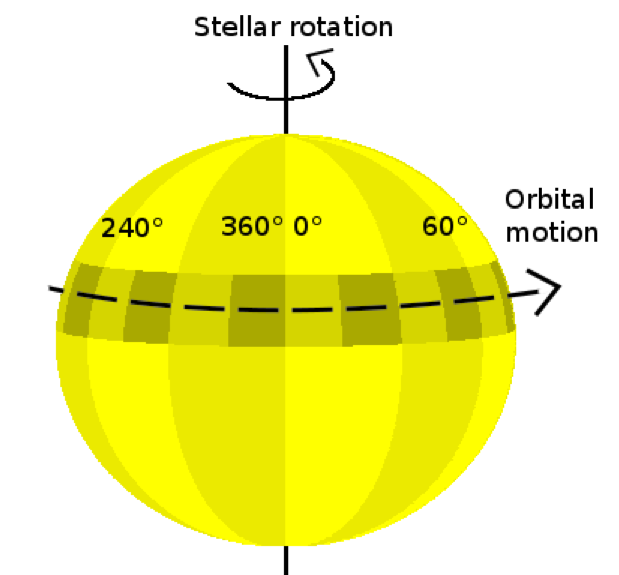
\includegraphics[width=.5\textwidth]{images/modelGeometry.png}
%	\caption{Example of a brightness map that is defined by our code. This image was taken from the first paper detailing this technique. It was done specifically on CoRoT 2.}
%	\label{CoRoT}
%\end{figure}
			
\subsection{Describe the inputs to the program}
	This section should describe the stellar input parameters, planetary input parameters, and the model input parameters.
	This will be a relatively short and straight-forward section.

\subsection{Model flux}
	This section should describe the general case for \fmod. It should also talk about the specific variables, $V_{i,j}$ and $b_j$ and motivate the reason for the visibility calculations below. It should describe the timescale for the evolution of starspots and our decision to include "windowing" in our model. And finally, it should give a brief description of the Simplex algorithm.
	
\section{Visibility as a function of time}
	This section should discuss all of the math involved in the visibility profile of a general case star.
%\begin{figure}[h]
%	\centering
%	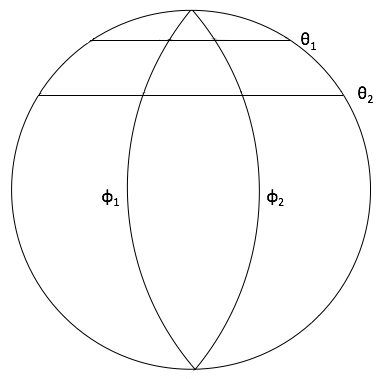
\includegraphics[width=.5\textwidth]{images/angles.png}
%	\caption{A reference image for the angles that are discussed in relation to the definition of visibility values on the star.}
%	\label{angles}
%\end{figure}
%\begin{figure}[h]
%	\centering
%	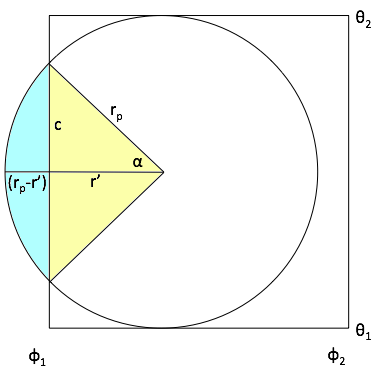
\includegraphics[width=.5\textwidth]{images/figure.png}
%	\caption{A simplified visualization of the geometry used in defining the eclipse path visibility of a system. The blue section is the important area for which we are solving.}
%	\label{eclipse}
%\end{figure}
%\begin{figure}[h]
%	\centering
%	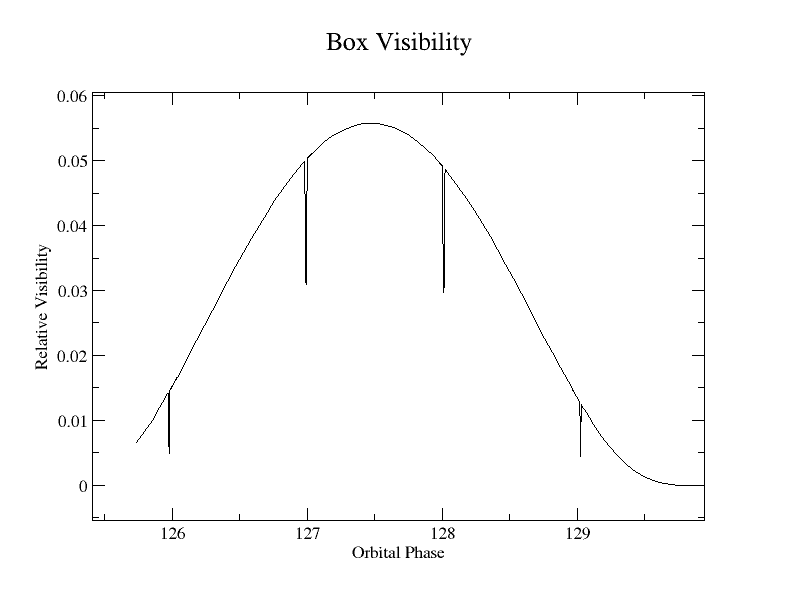
\includegraphics[width=.5\textwidth]{images/box_vis.png}
%	\caption{The visibility of one box during one window. Note that the transit dips are not full transits, but only a portion of the transit while the planet is in front of that specific region.}
%	\label{box}
%\end{figure}

	
\subsection{Region Visibilities}
	This should outline the rationale behind the integral used to calculate the projected surface area of each region. It should show the integral once and then show that for a box and a longitude, the $\theta$ limits are the only thing that change. It should also discuss the fact that the stripe visibilities are calculated within the Amoeba Algorithm and why (or I should change it in the code).
	
\subsection{Transiting Planet Model}
	This section should discuss the idea that the planet is nothing more than a blocking of visibility while it is occluding the star. It should explain the basic geometry of this calculation and show the ten different cases involved.

\subsection{Limb Darkening}
	The final visibility section will outline the limb darkening. Important facts to include are that we use a quadratic limb darkening equation, we include limb darkening both in and out-of-transit, and the specific math behind our calculations for each region (yay for analytically solving things).

\textbf{Note}

Everything is done as a function of time over the orbit.

\section{Validating our Model}
Now that we have properly defined how our model works theoretically, we need to prove that it does work in practice
\subsection{What is variable?}
	Give a description of the parameters that we still can mess with. For example, the number of stripes, number of boxes,  and binning cadences both in and out-of-transit.
\subsection{Making the model light curves}
	Describes the process of generating a model light curve and how, in our case, it was intrinsically linked to the stellar and planetary parameters of Kepler 17. It should briefly mention that I use a python script to generate Gaussian noise based on Kepler magnitude noise. It should also outline the list of spot models that we tried and our motivation for doing so.
	
%\begin{figure}[h]
%	\centering
%	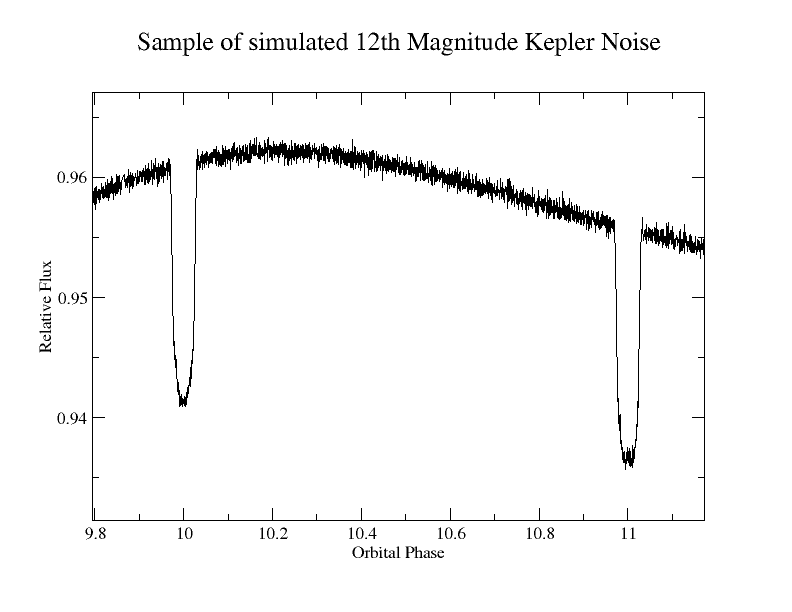
\includegraphics[width=.5\textwidth]{images/12_noise.png}
%	\caption{Example of Gaussian noise in a model. This particular light curve part is one "window" in our model. It has a simulated noise similar to that of a Kepler 12th magnitude star.}
%	\label{noise}
%\end{figure}

\subsection{Testing Complexity}
We have only tested the ability of our program to solve for brightness values in two parameter spaces, complexity of the spots and noise of the light curve.

\subsection{Results}
Show plots (RMS, 2d boxes over time, stripes, etc.)
%\begin{figure}[h]
%	\centering
%	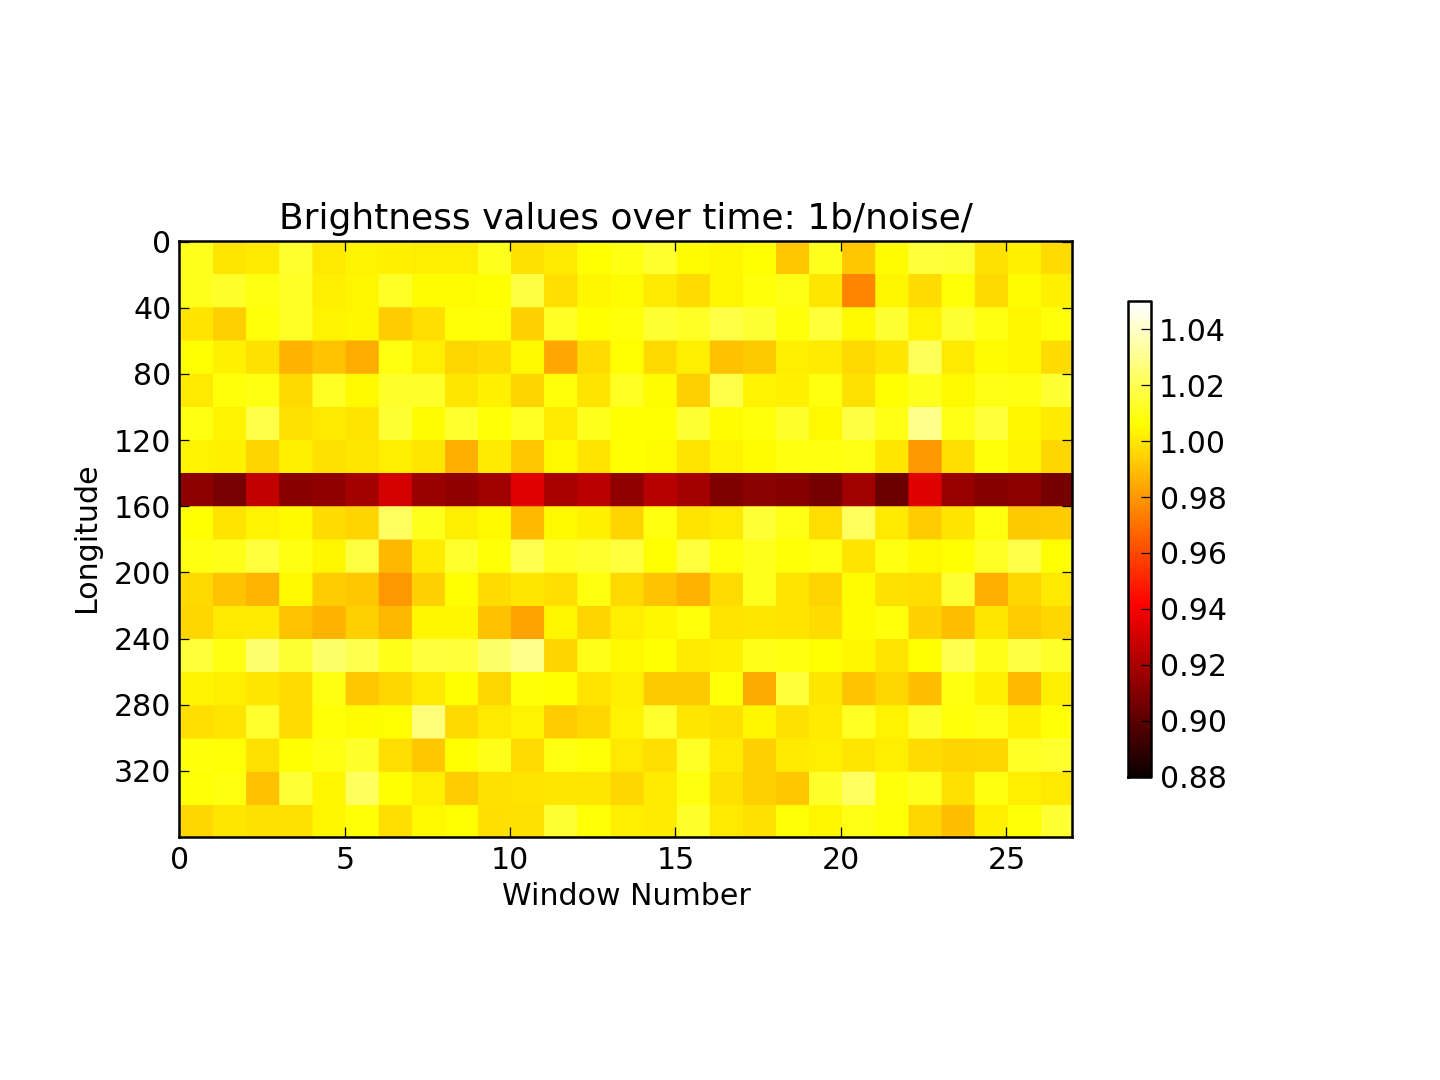
\includegraphics[width=.5\textwidth]{images/1b/noise/region_plot.png}
%	\caption{Boxes over multiple trials for 1 box}
%	\label{1b/noise}
%\end{figure}
%\begin{figure}[h]
%	\centering
%	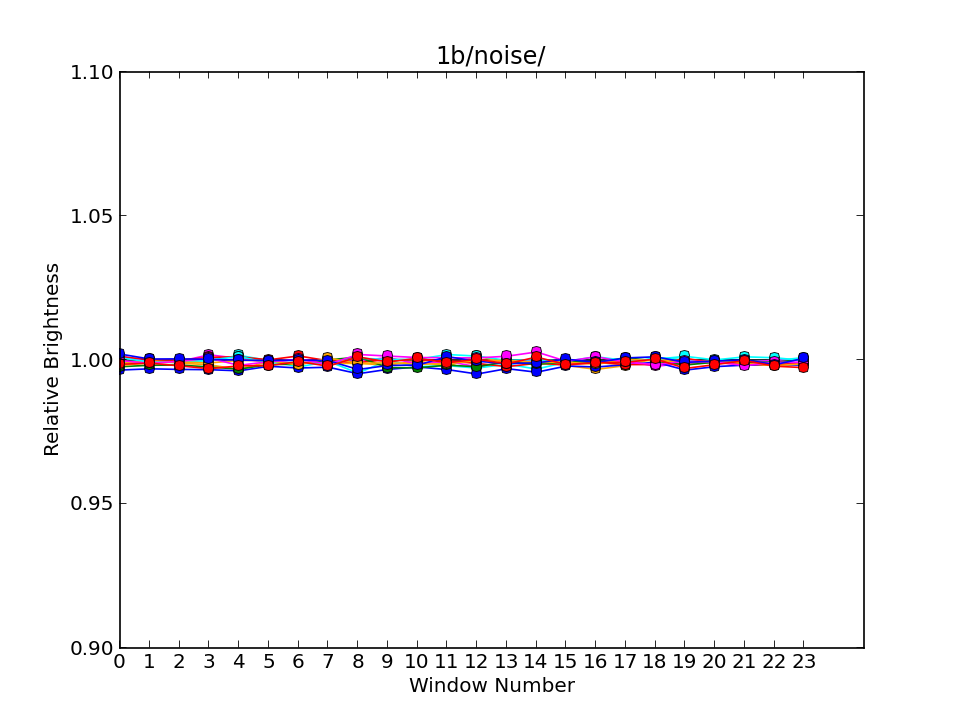
\includegraphics[width=.5\textwidth]{images/1b/noise/stripes_over_time.png}
%	\caption{Stripes over multiple trials for 1 box}
%	\label{1b/noise/stripes}
%\end{figure}
%
%\begin{figure}[h]
%	\centering
%	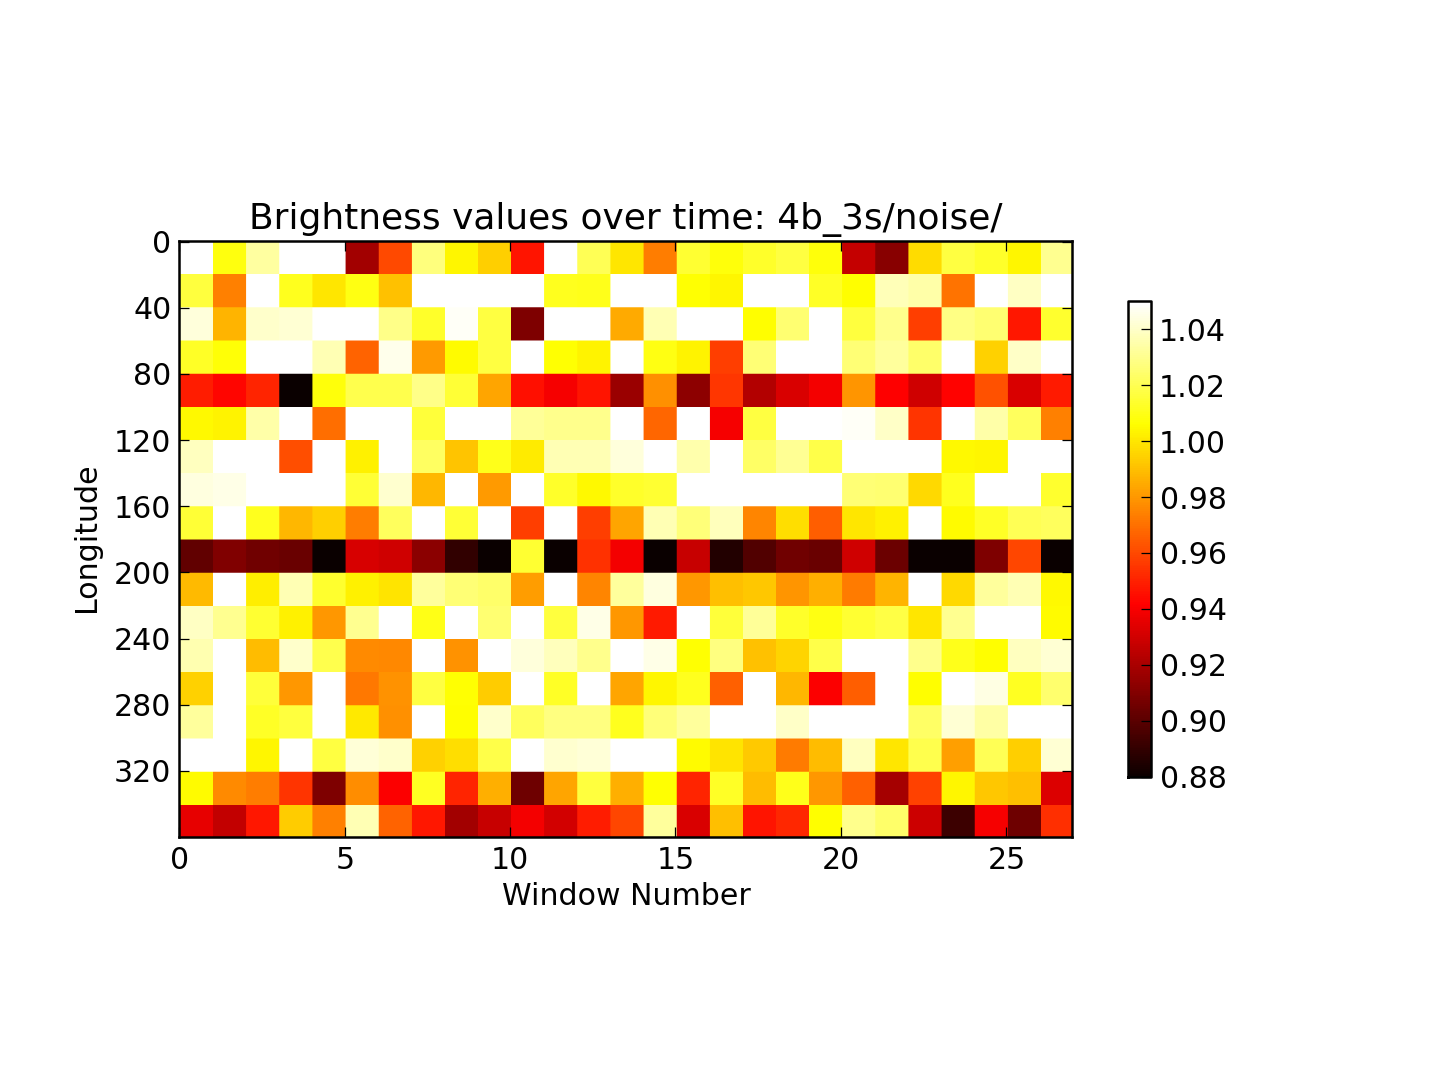
\includegraphics[width=.5\textwidth]{images/4b_3s/noise/region_plot.png}
%	\caption{Boxes over multiple trials for 4 boxes and 3 stripes}
%	\label{4b_3s/noise}
%\end{figure}
%\begin{figure}[h]
%	\centering
%	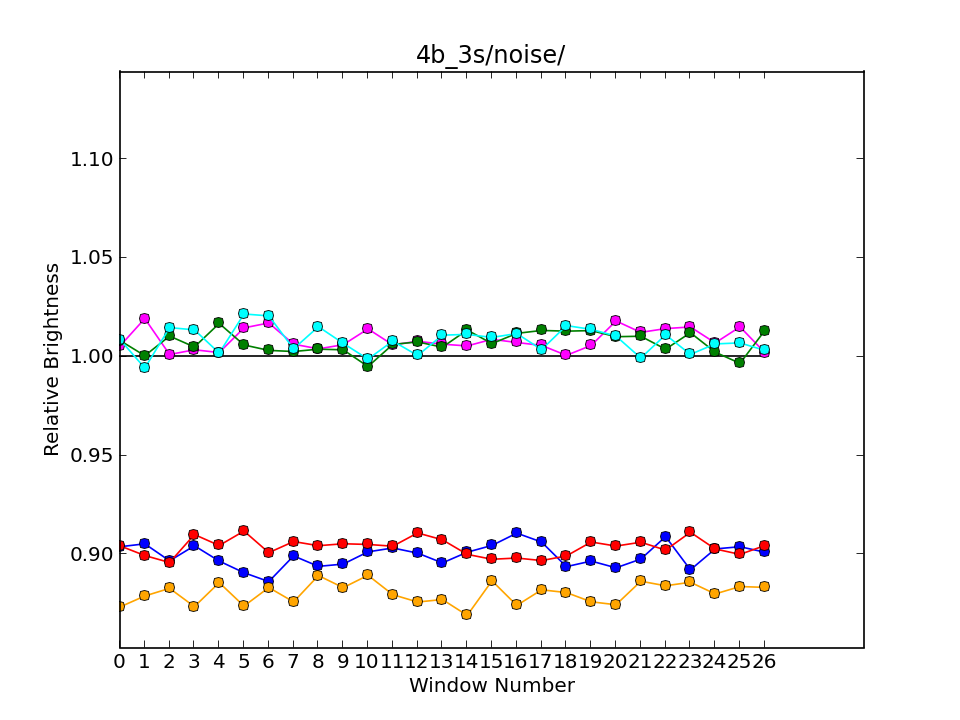
\includegraphics[width=.5\textwidth]{images/4b_3s/noise/stripes_over_time.png}
%	\caption{Stripes over multiple trials for 4 boxes and 3 stripes}
%	\label{4b_3s/noise/stripes}
%\end{figure}
%
%\begin{figure}[h]
%	\centering
%	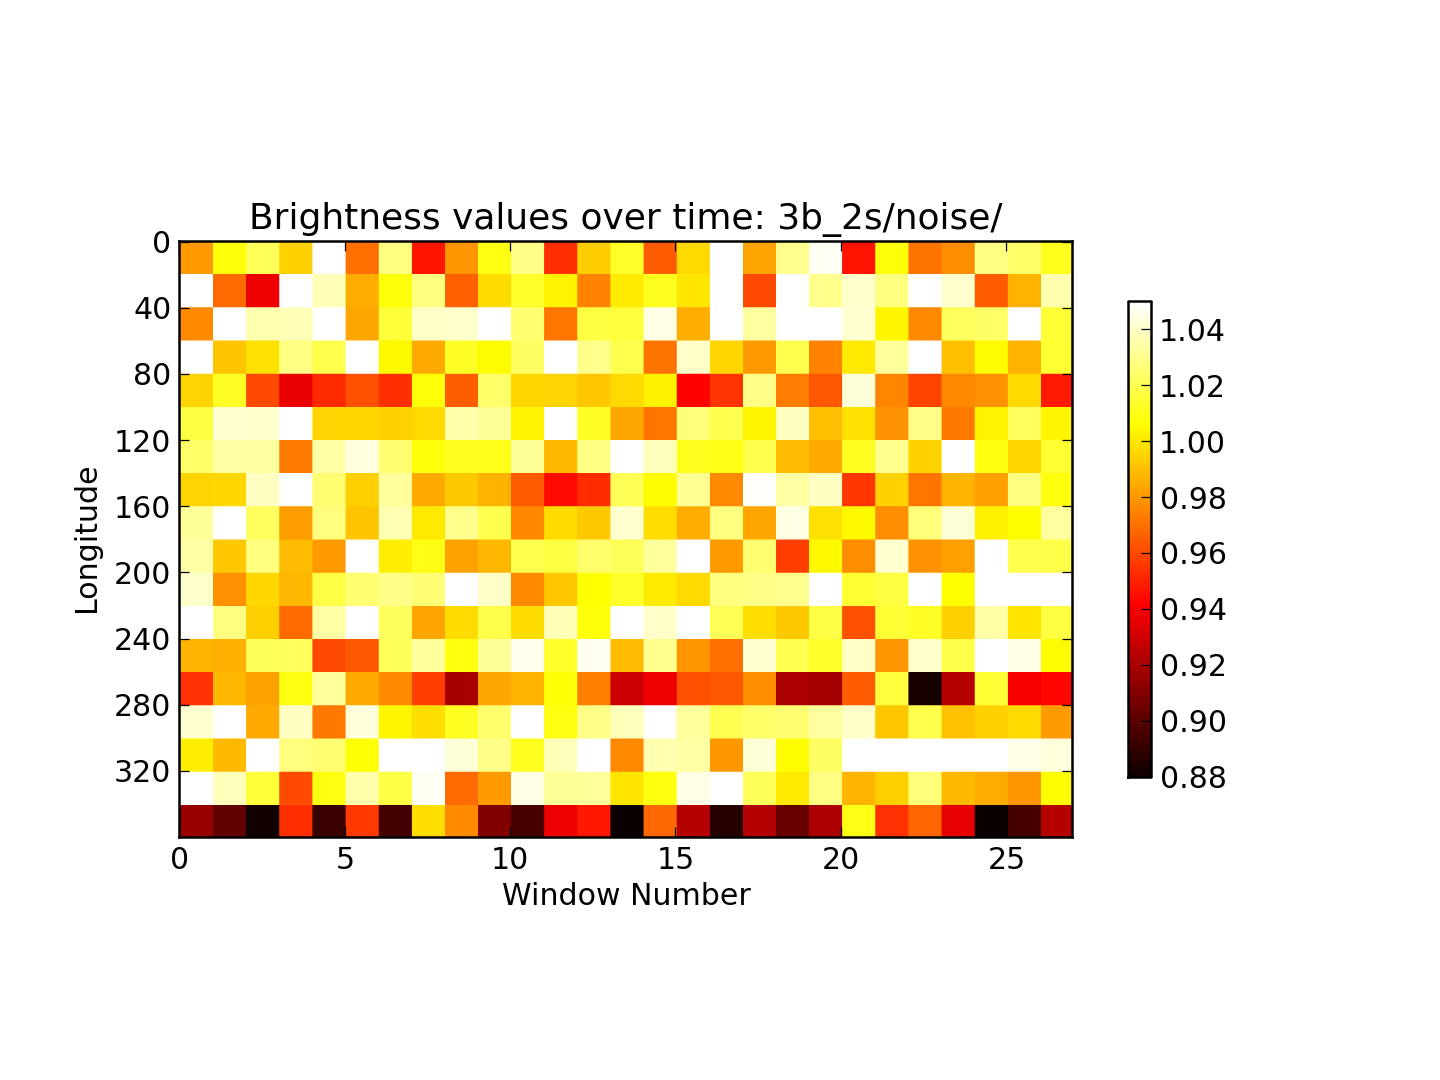
\includegraphics[width=.5\textwidth]{images/3b_2s/noise/region_plot.png}
%	\caption{Boxes over multiple trials for 3 boxes and 2 stripes}
%	\label{3b_2s/noise}
%\end{figure}
%\begin{figure}[h]
%	\centering
%	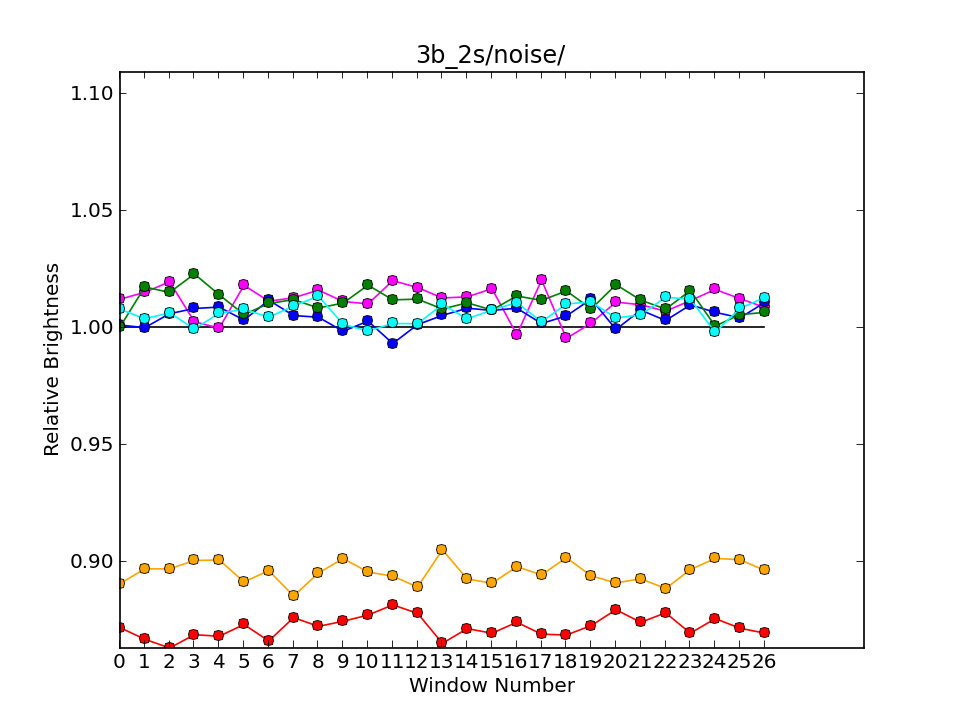
\includegraphics[width=.5\textwidth]{images/3b_2s/noise/stripes_over_time.png}
%	\caption{Stripes over multiple trials for 3 boxes and 2 stripes}
%	\label{3b_2s/noise/stripes}
%\end{figure}
%
%\begin{figure}[h]
%	\centering
%	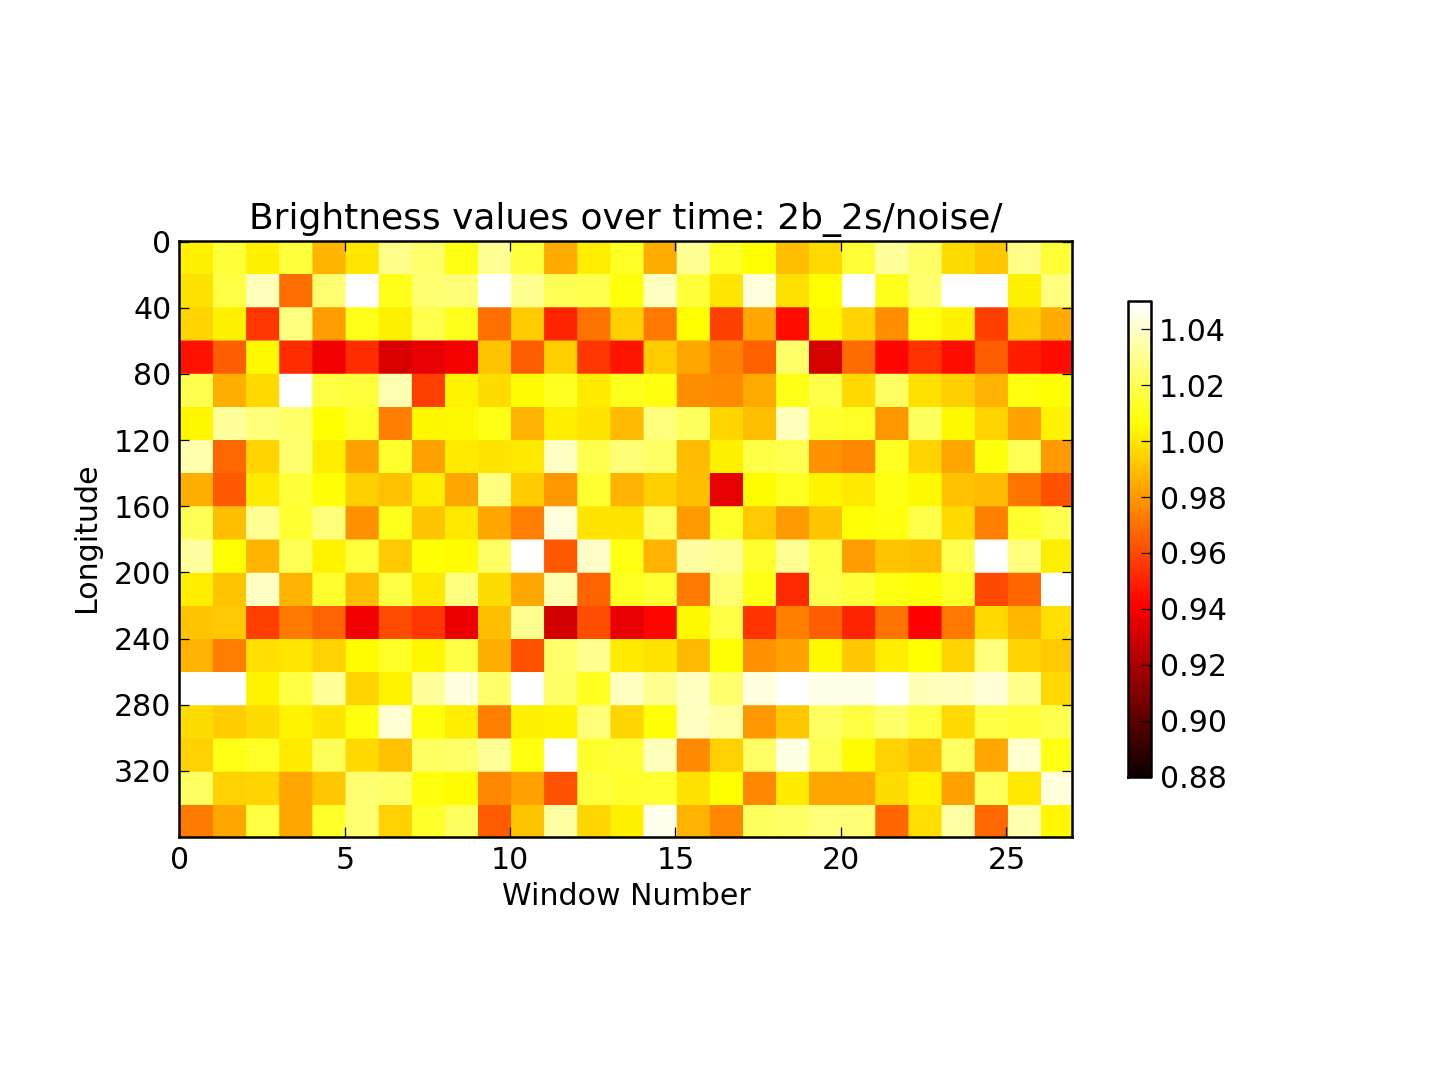
\includegraphics[width=.5\textwidth]{images/2b_2s/noise/region_plot.png}
%	\caption{Boxes over multiple trials for 2 boxes and 2 stripes}
%	\label{2b_2s/noise}
%\end{figure}
%\begin{figure}[h]
%	\centering
%	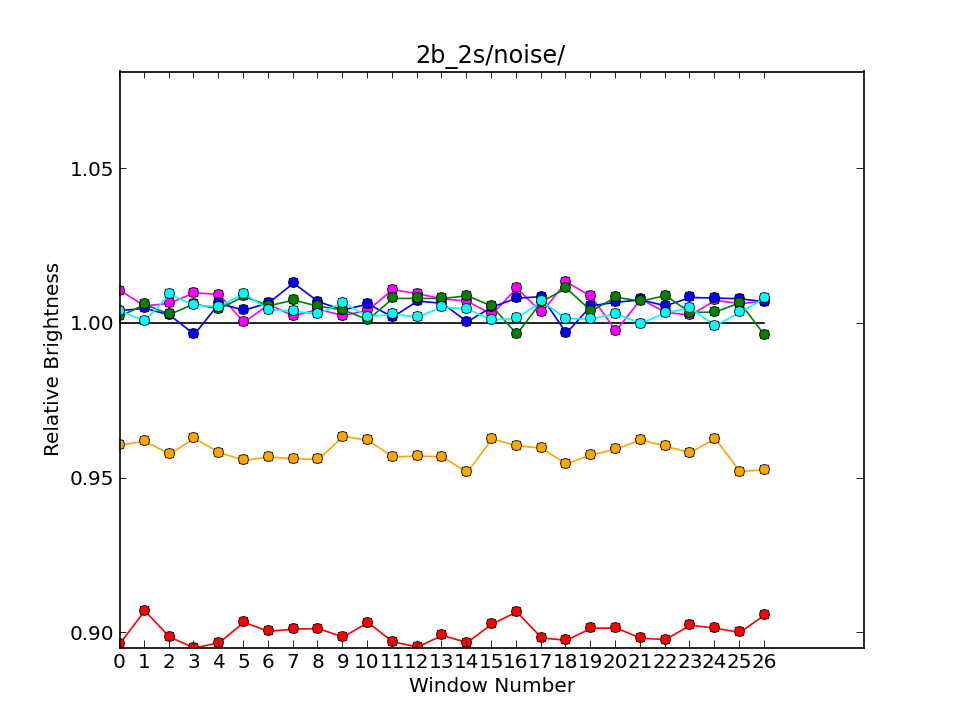
\includegraphics[width=.5\textwidth]{images/2b_2s/noise/stripes_over_time.png}
%	\caption{Stripes over multiple trials for 2 boxes and 2 stripes}
%	\label{2b_2s/noise/stripes}
%\end{figure}
%\begin{figure}[h]
%	\centering
%	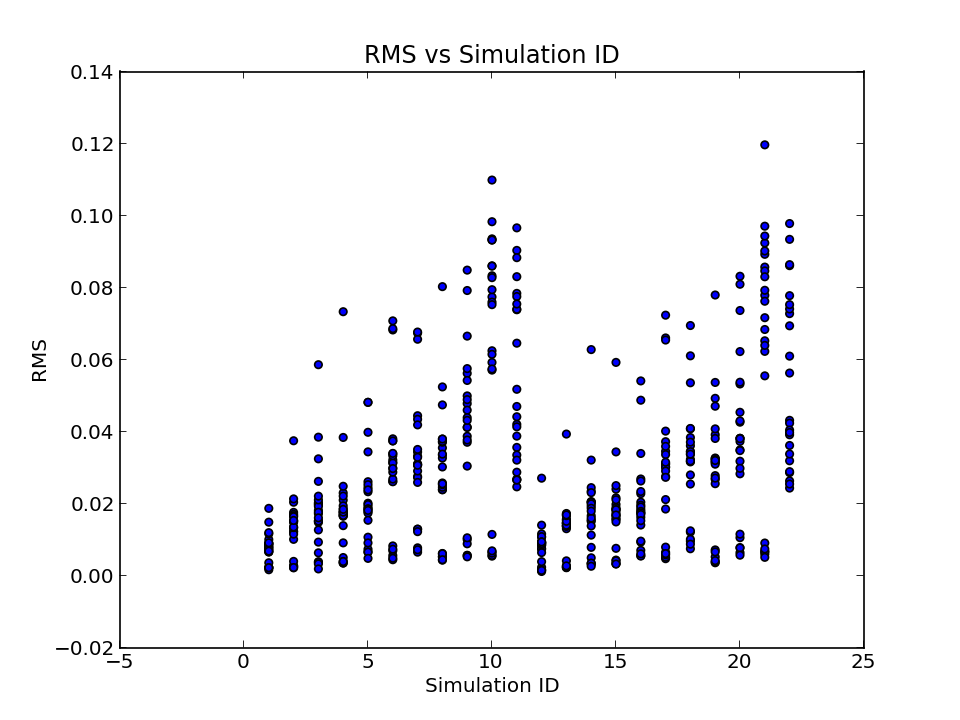
\includegraphics[width=.5\textwidth]{images/rms_over_time.png}
%	\caption{RMS of the model light curve brightness inputs to the recovered value for each type of simulation over all windows}
%	\label{RMS}
%\end{figure}	

\section{Application of our program to real data}
Kepler 17





\section{Possible Figures \label{figures}}
	\begin{enumerate}
		\item Brightness maps
		\item Model lightcurve fits
		\item Stripes over time
		\item Boxes over time
		\item Errors and residuals
		\item Unbinned vs. binned lightcurves
		\item \ldots?
	\end{enumerate}
\end{document}